% !Mode:: "TeX:UTF-8"
% !TEX program  = xelatex
\title{Assignment 2}
\maketitle\tableofcontents

\section{Question 1}
\begin{statebox}{}{question-1}
    Suppose that for the same asset and expiry date, you hold a European call option with exercise price $E_1$ and another with exercise price $E_3$, where $E_3>E_1$ and also write two calls with exercise price $E_2:=(E_1+E_3)/2$. Derive a formula for the value at expiry and draw the corresponding payoff diagram. Write a code to verify it.
\end{statebox}
I use $V_h$ to represent two European call options that we hold, $V_w$ to represent two calls that we write, and $S_T$ to represent the exercise price. Therefore, we have
\begin{equation}\label{E:value-at-expiry-1}
    \begin{aligned}
        V_h &= \max(S_T-E_1, 0) + \max(S_T-E_3, 0) \\
        V_w &= E_2 - \max(S_T-E_2, 0).
    \end{aligned}
\end{equation}

That is,
\begin{equation}\label{E:value-at-expiry-2}
    V = V_h + 2V_w = \begin{cases}
        E_1+E_3 & \text{where } S_T\leq E_1, \\
        S_T+E_3 & \text{where } E_1<S_T\leq E_2, \\
        E_1+2E_3-S_T & \text{where } E_2<S_T\leq E_3, \\
        E_1+E_3 & \text{where } E_3<S_T.
    \end{cases}
\end{equation}

The payoff diagram of $E_1=2$ and $E_3=4$ is Figure~\ref{F:payoff-diagram}.
\begin{figure}[H]
    \centering
    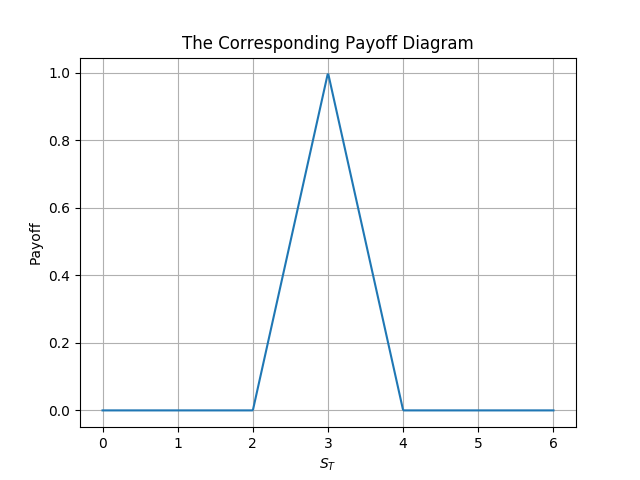
\includegraphics[width=.7\textwidth]{figures/2019-09-27-payoff-diagram.png}
    \caption{Payoff Diagram}\label{F:payoff-diagram}
\end{figure}

And the code that verifies the result shows below.
\Python{Verification}{code/2-1.py}



\section{Question 2}
\begin{statebox}{}{question-2}
    Find a systematic way to construct a portfolio of options with arbitrary payoffs.
\end{statebox}
假设我们希望的收益位于$(x,y)$,如果$y$小于0,我们过收益点做斜率为$-1,-2,\ldots$的直线,直到直线交$x$轴于正半轴;如果$y$大于0,我们过收益点做斜率为$1,2,\ldots$的直线,直到直线交$x$轴于正半轴。此时直线斜率为我们需要购买期权的最小数量,而与$x$轴正半轴所交点即为$E$值(当然不唯一)。

根据期权收益公式可以有如下代码,将期权的特点抽象出来,收益图展示见图~\ref{F:payoff-diagram-2}。
\begin{figure}[H]
    \centering
    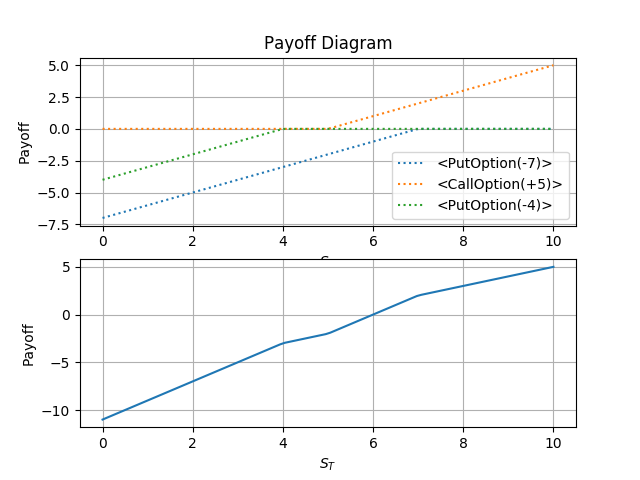
\includegraphics[width=.7\textwidth]{figures/2019-09-27-payoff-diagram-2.png}
    \caption{Payoff Diagram}\label{F:payoff-diagram-2}
\end{figure}
\Python{Option API}{code/2-2.py}



\section{Question 3}
\begin{statebox}{}{question-3}
    Find all types of options in major global trade market.
\end{statebox}
\begin{itemize}
    \item 行权时间:
        \begin{itemize}
            \item 欧式期权,行权时间较固定;
            \item 美式期权,行权时间较宽松;
            \item 百慕大期权,可以在到期日前所规定的一系列时间行权。
        \end{itemize}
    \item 期权权利:
        \begin{itemize}
            \item 看涨期权;看跌期权。
        \end{itemize}
    \item 合约标的
        \begin{itemize}
            \item 现货期权(股票、股指、利率、外汇);商品期权。
        \end{itemize}
    \item 行权价格与标的证券市价的关系
        \begin{itemize}
            \item 实值期权;平值期权;虚值期权。
        \end{itemize}
\end{itemize}



% \bibliography{ref}
